\section{Introducción}
\vspace{0.2cm}
\noindent En esta práctica vamos a hacer una síntesis del ácido acetilsalicílico (también conocido como Aspirina) partiendo de ácido salicílico, es un proceso fácil pero requiere bastante tiempo y atención. \\\\
A lo largo de esta práctica prepararemos disoluciones, las trabajaremos al baño maría y pasaremos un par de veces por el proceso de cristalización que lo podemos ver visualmente en la Figura \ref{fig:cris}.

\vspace{0.4cm}

\begin{figure}[h]
    \centering
    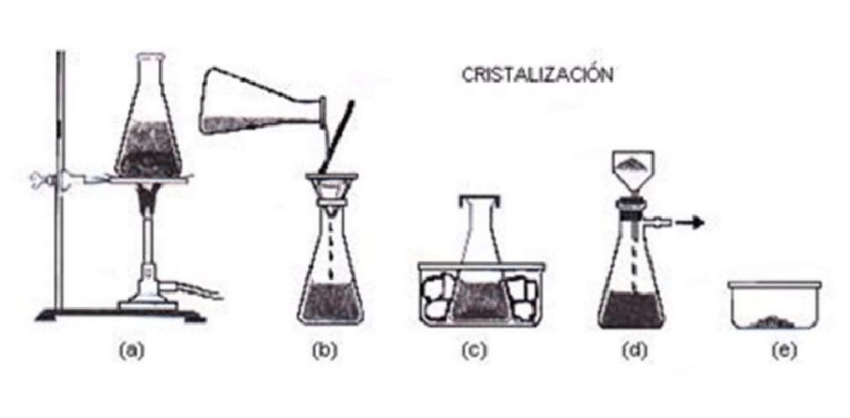
\includegraphics[scale = 0.5]{Figura-3-Proceso-general-de-cristalizacion-por-pasos-Fuente.png}
    \caption{Imagen de un proceso de cristalización}
    \label{fig:cris}
\end{figure}

\vspace{0.6cm}

\noindent En el apartado \ref{proc} explicaremos más detalladamente el desarrollo de la práctica.

\clearpage
\section{Inventario}  
\noindent En esta práctica contamos con:
\begin{multicols}{2}
    \begin{itemize}
        \item 4 tubos de ensayo 
        \item 1 picnómetro
        \item 3 vasos de precipitados
        \item Un erlemmeyer
        \item 2 pipetas
        \item Una varilla
        \item Una probeta
        \item Un frasco lavador
        \item Un matraz Kitasatos
        \item Un embudo Büchner
        \item 2 vidrios de reloj
        \item Una placa calefactora
        \item Una espátula
        \item Una báscula
        \item Un matraz cristalizador
        \item Un termómetro
        \item Etanol
        \item Tricloruro de hierro
        \item Ácido salicílico
        \item Unos guantes de silicona
    \end{itemize}
\end{multicols}

\vspace{0.8cm}
\noindent Como bien podemos ver en las siguientes fotografías.
\vspace{0.4cm}

\begin{figure}[h]
    \centering
    \hspace*{-2.3cm}
        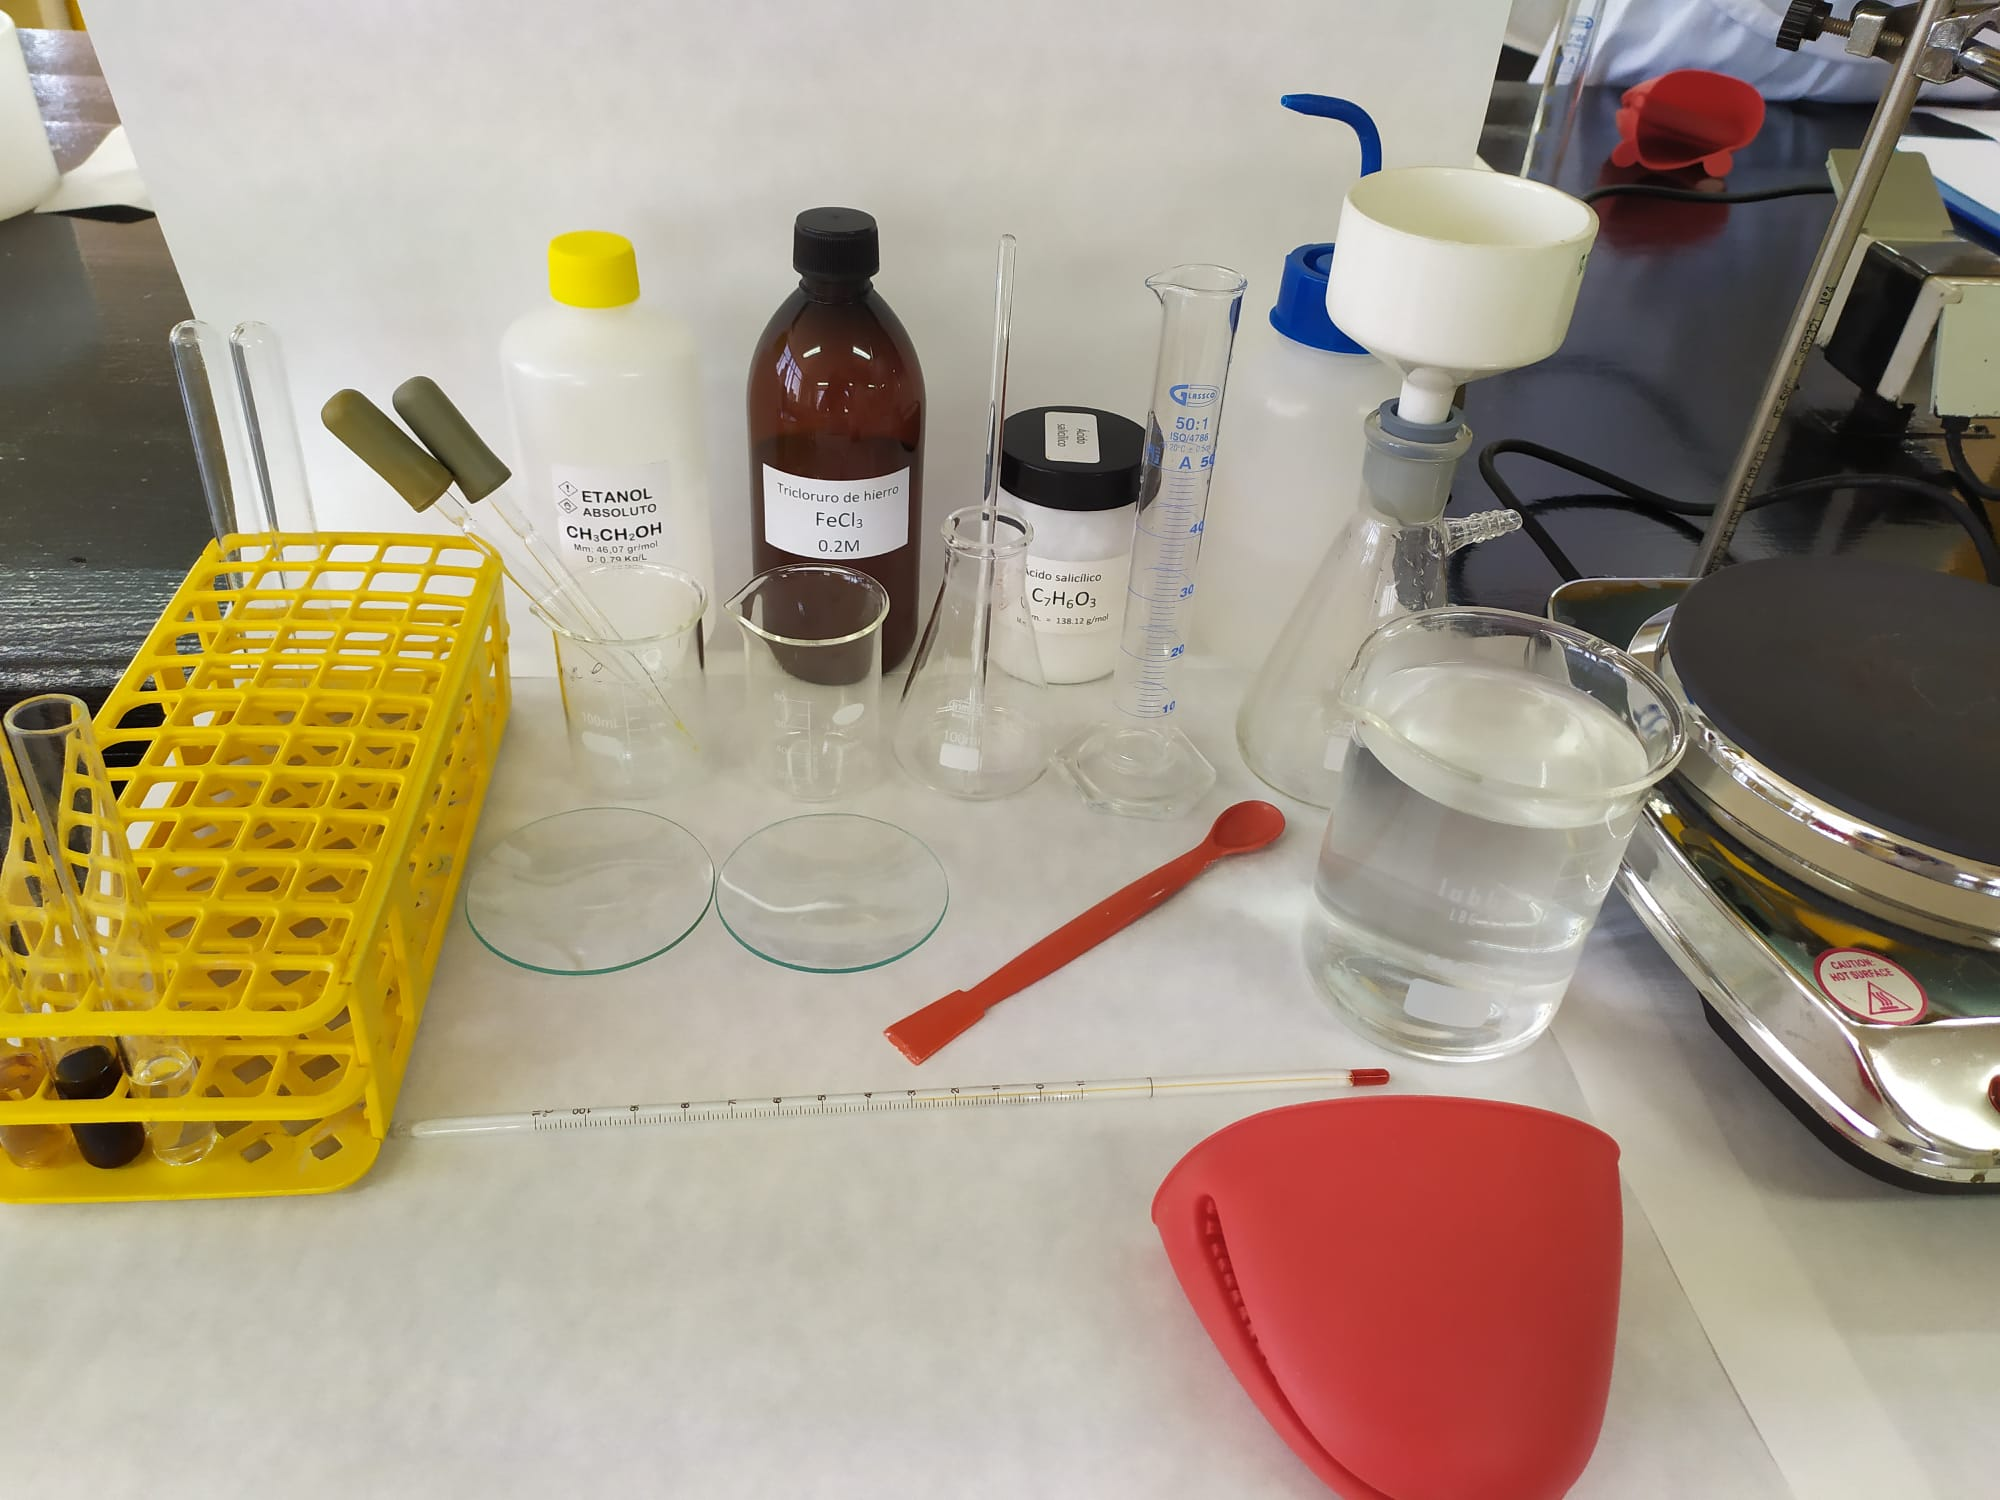
\includegraphics[scale = 0.1]{fotos/set6-1.jpeg}
        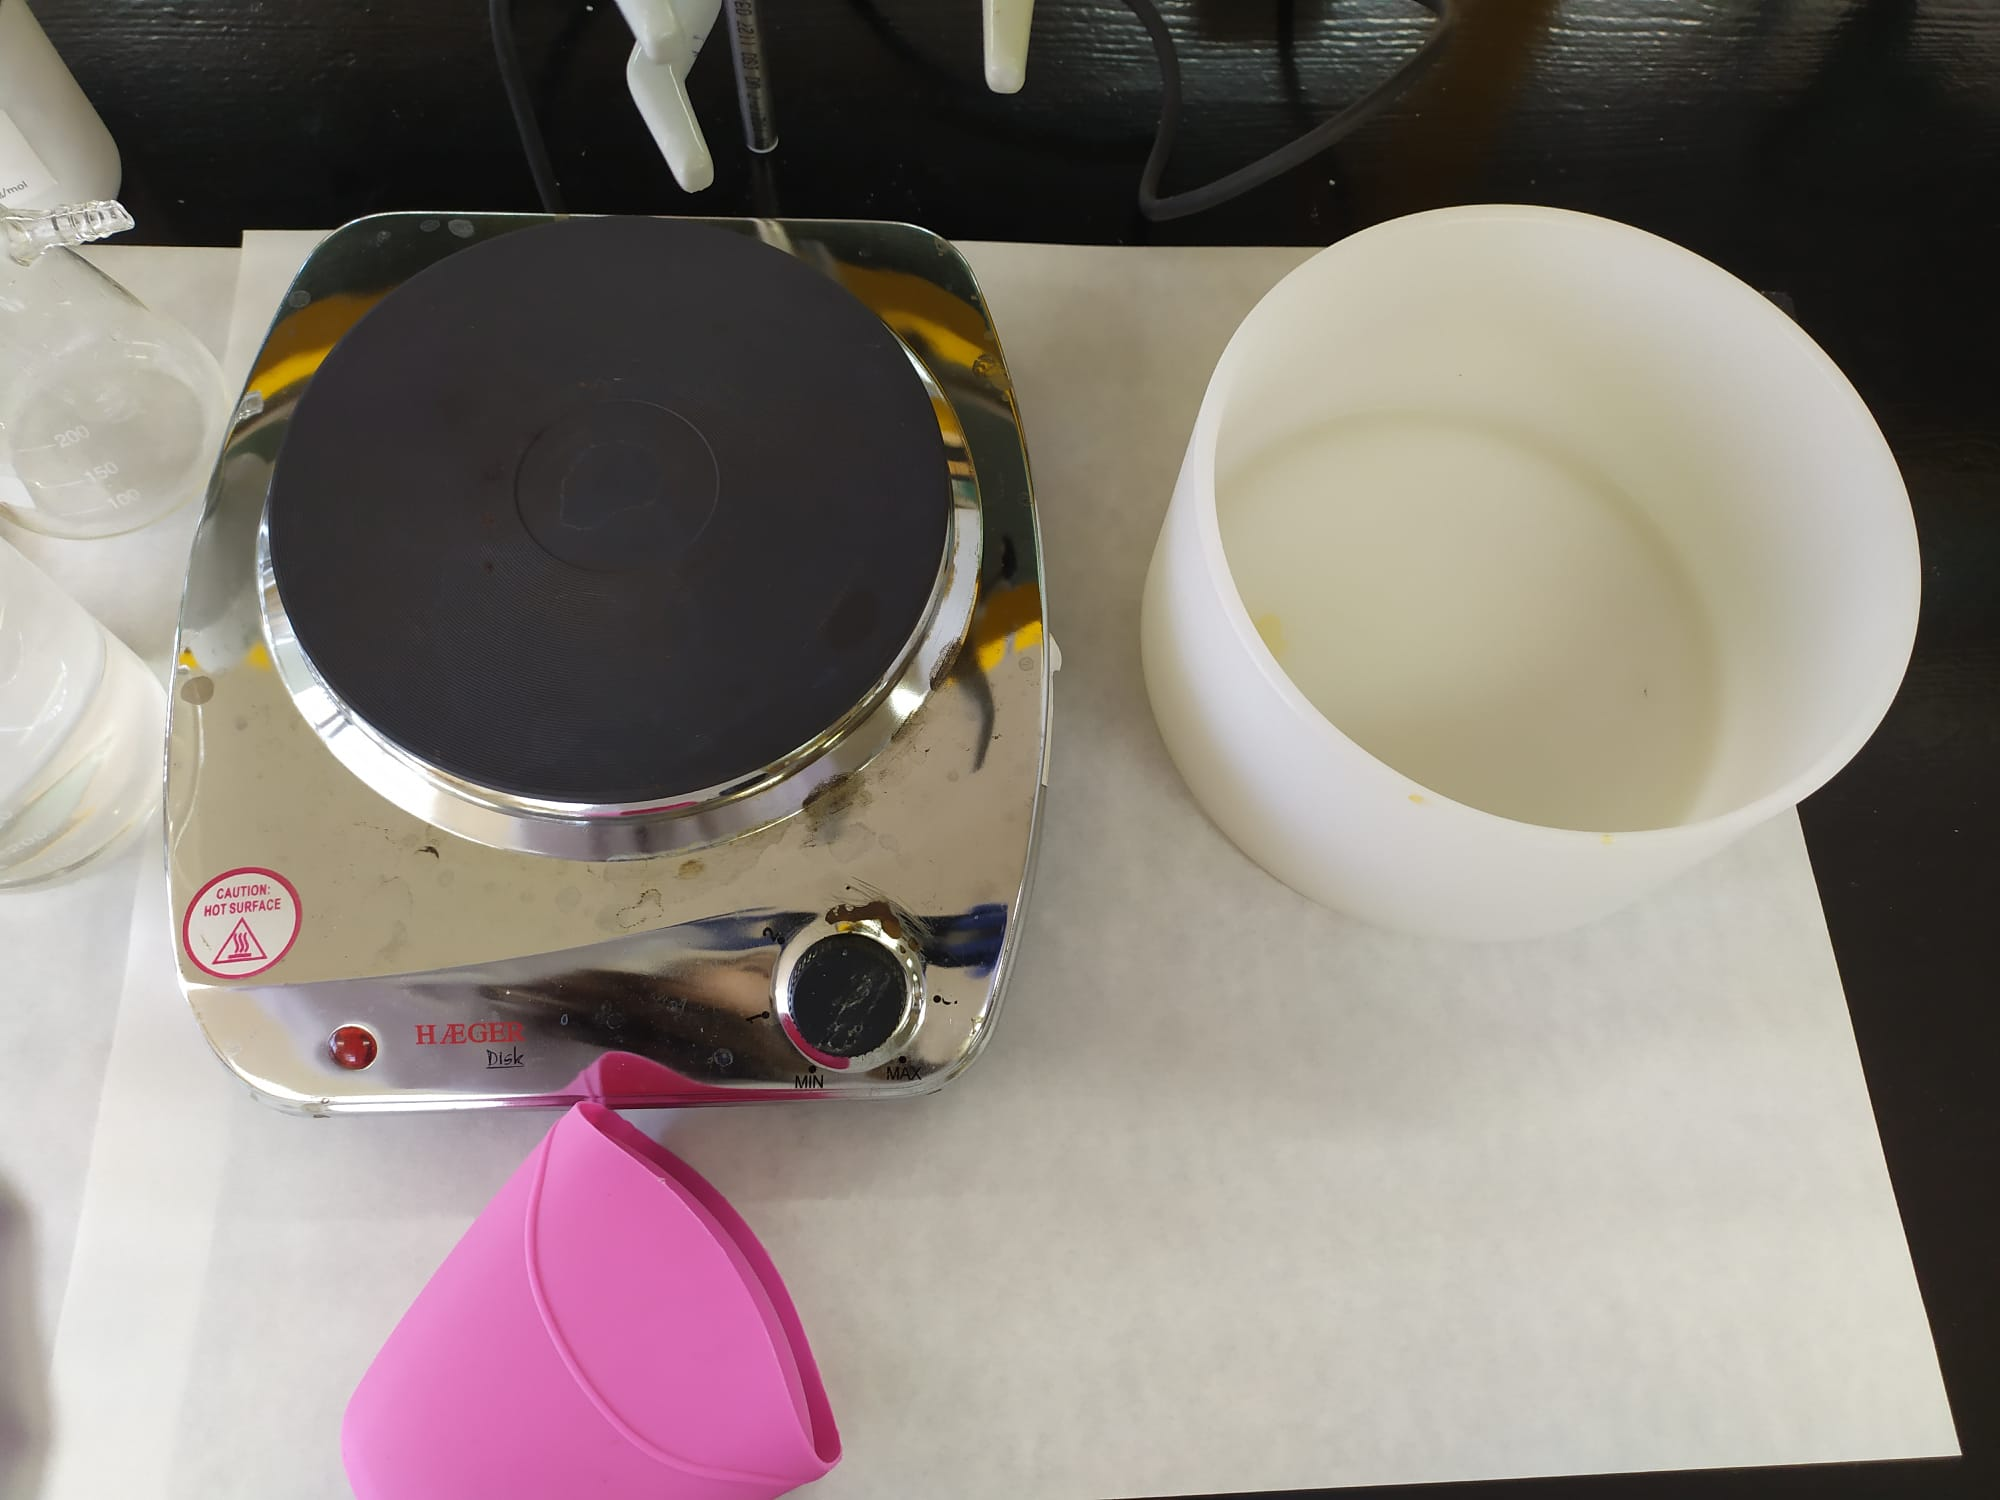
\includegraphics[scale = 0.1]{fotos/set6-2.jpeg}
    \hspace*{-2.3cm}
    \caption{Material de la práctica}
\end{figure}

\clearpage

\section{Procedimiento}\label{proc}
\noindent En primer lugar, tenemos que poner a calentar un vaso grande con agua en la placa calefactora para poder usar el baño maría. Cuando esté muy caliente pero sin necesidad de hervir, pondremos la disolución previamente preparada: hemos pesado 6g exactos de ácido salicílico en un matraz erlenmeyer y le hemos añadido 8 mL de anhídrido acético y 10 gotas de ácido sulfúrico concentrado. 

\vspace{0.2cm}

\noindent Una vez puesta la disolución al baño maría, la tendremos ahí alrededor de unos 20 minutos mientras que con una varilla la vamos removiendo para conseguir completar la reacción de la mezcla.

\vspace{0.2cm}

\noindent Tras los 20 minutos, agregamos poco a poco 25 mL de agua muy fría (destilada), para después ponerlo en el matraz cristalizador con hielo picado durante unos 10 minutos, hasta que la precipitación se complete.

\vspace{0.2cm}

\noindent Una vez se da la cristalización, separamos el precipitado del líquido mediante filtración al vacío durante 10 minutos más o menos. También lavaremos con agua fría el precipitado para que sea lo más puro posible.

\vspace{0.2cm}

\noindent A continuación, separaremos un poco de precipitado para realizar la prueba de fenoles al final de la práctica y el resto lo pasaremos a un vaso de precipitados de 100 mL para disolverlos con 15 mL de alcohol etílico para volver a calentarlo al baño maría hasta que ya no veamos el precipitado. Mientras hacemos esto, calentamos 50 mL de agua (destilada). Una vez sacado el vaso de precipitados le añadimos el agua que estábamos calentando, y cubrimos la disolución con un vidrio reloj (colocado como en la Figura \ref{fig:prec} hasta que se enfríe la mezcla y que consigamos una completa cristalización. Nosotros en un principio la dejamos enfriar a temperatura ambiente, pero debido al lento proceso, lo metimos en el cristalizador con hielo picado para que el proceso de precipitación tuviera lugar más rápidamente.


\vspace{0.4cm}

\begin{figure}[h]
    \centering
    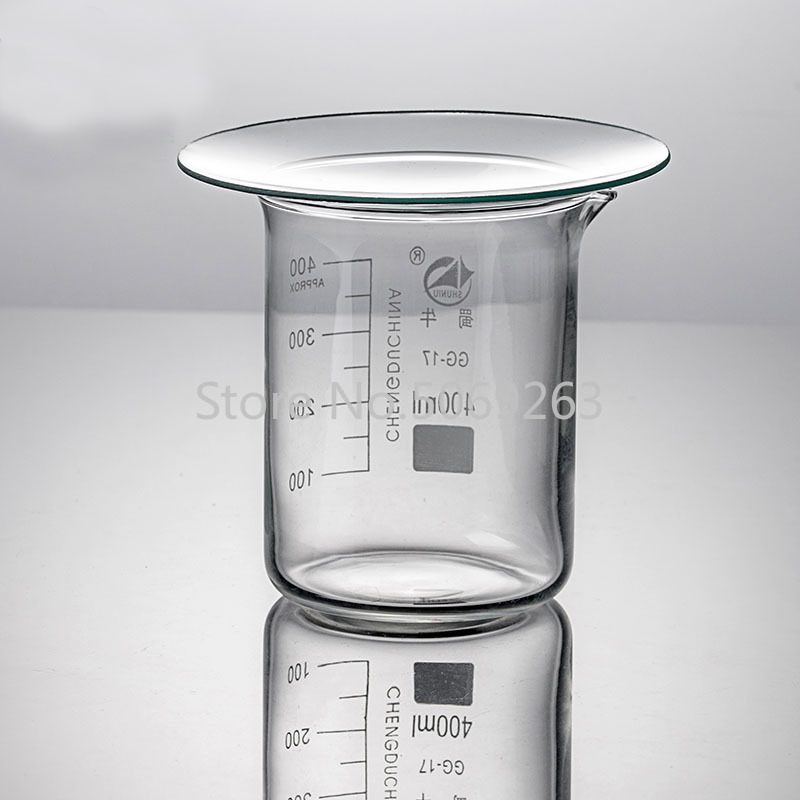
\includegraphics[scale = 0.12]{fotos/Plato-de-reloj-de-vidrio-de-laboratorio-cubierta-de-vaso-duro-en-forma-de-c-pula.jpg}
    \caption{Imagen de un vaso de precipitados con un vidrio reloj}
    \label{fig:prec}
\end{figure}

\vspace{0.4cm}

\noindent Una vez precipitado, volvemos a filtrar al vacío y los cristales formados los pasamos a un vaso limpio, y que ya hemos pesado (34.77 g), para después meterlo a la estufa con la finalidad de secar los cristales de ácido acetilsalicílico. Sacaremos el vaso de precipitados cada 5 minutos para pesarlo, hasta que dicho peso sea constante (esto último no vamos a poder hacerlo bien ya que para que la pesada sea constante tendríamos que esperar por lo menos hasta el día siguente).

\vspace{0.3cm}

\begin{table}[h]
    \centering
\begin{tabular}{ | c | c | } 
    \hline
    \multicolumn{2}{ |c| }{Resultados} \\
    \hline
    $T_1$ $(g)$ & 39.72 \\  
    $T_2$ $(g)$ & 39.6 \\  
    $T_3$ $(g)$ & 39.49 \\  
    $T_4$ $(g)$ & 39.35 \\  
    $T_5$ $(g)$ & 39.23 \\  
    $T_6$ $(g)$ & 39.12 \\  
    $T_7$ $(g)$ & 39.05 \\  
    \hline
\end{tabular}
    \caption{Tabla de los datos obtenidos  tras las mediciones}
    \label{tabla-gramos}
\end{table}

\vspace{0.3cm}

\noindent Por último, vamos a realizar la prueba de los fenoles. Para ello disolveremos en tres tubos de ensayo que ya contengan 5 mL de etanol algunos cristales de ácido salicílico (1), en otro tubo el producto sin purificar que habíamos reservado (2) y otro con el producto purificado obtenido al finalizar la práctica (3). Y les añadimos tres gotas de tricloruro.

\vspace{0.2cm}

-- En el \textbf{primer tubo} de ensayo obtenemos un color morado intenso porque reacciona con el ácido salicílico dando lugar a ese característico color.

\vspace{0.15cm}

-- En el \textbf{segundo tubo} encontraremos también un toque morado, pero prácticamente incoloro, ya que aún tenemos impurezas.

\vspace{0.15cm}

-- En el \textbf{tercer tubo} ya no hay casi morado, pero aún se aprecia un poco porque no hemos terminado correctamente el proceso y hay impurezas de ácido salicílico, que es lo que reacciona.



\vspace{0.2cm}
\noindent Por tanto, hemos conseguido llegar casi al ácido acetilsalicílico pero en esta prueba hemos podido observar que aún nos quedaría dejar la muestra más tiempo en la estufa.

\clearpage

\section{Cuestiones} 

\noindent Empezamos con 6 gramos de ácido salícilico, y terminamos con $\approx$ 3 gramos de ácido acetilsalicílico, por tanto obtenemos un rendimiento del 50$\%$

\vspace{0.3cm}

\noindent La reacción que se produce es $C_7H_6O_3 + C_4H_6O_3 \rightarrow C_9H_8O_4 + C_2H_4O_2$, y podemos observar que un mol de ácido salicílico reacciona con un mol de ácido acetilsalicílico, y sabemos que la masa final de producto es 39.05 - 34.77 = \underline{4.28 g}. Para calcular la masa teórica (para así sacar el rendimiento) deberemos pasar los 6 gramos iniciales de ácido salicílico a los gramos finales de ácido acetilsalicílico mediante factores de conversión:

\vspace{0.3cm}

\noindent Sabiendo que la masa molar de ácido acetilsalicílico es de 180 g/mol y la del ácido salicílico es de 138 g/mol ya podemos calcular la masa teórica:

\[ 6 ~ g \cdot \frac{1 ~ mol ~ C_7H_6O_3}{102 ~ g ~ C_7H_6O_3} \cdot \frac{180 ~ g ~ C_9H_8O_4}{1 ~ mol ~ C_9H_8O_4} = 7.82 ~ g ~ de ~ C_9H_8O_4\]

\noindent Una vez hallada la masa teórica, ya podemos calcular el rendimiento:

\[ Rendimiento = \frac{masa ~ real}{masa ~ teorica}\cdot{100} = \frac{4.28}{7.82}\cdot{100} = 54.73\% \]


\vspace{0.3cm}

%%%%%%%%%%%%%%%%%%%%%%%%%%VEEEEEEEEEEEEEERRRRRRRRRR

\noindent Podemos observar que hemos perdido casi la mitad de la masa inicial, debido a que el proceso ha sido más rápido de lo que debería, tendríamos que dejarlo una noche entera.


%%%%%%%%%%%%%%%%%%%%%%%%%%VEEEEEEEEEEEEEERRRRRRRRRR







